\chapter{Desenvolvimento do Jogo}\label{ch:Desenvolvimento}

%A documentação do jogo é o Game Design Document (ou GDD para os íntimos). Alguns chamam também de Game Design Bible. É a mesma coisa

O processo de desenvolvimento de jogos digitais é uma tarefa que exige do(s) desenvolvedor(es) conhecimentos de programação. Um jogo para ser desenvolvido, deve ser escrito em uma determinada linguagem de programação, o que acaba por obrigar que o(s) desenvolver(es) do jogo tenha(m) conhecimento sobre esta linguagem. Embora existam linguagens de programação visual, o conhecimento sobre lógica de programação ainda é parte fundamental para o desenvolvimento de um jogo. 

%(programação em blocos ou Visual Scripting) : linguagem de programação visual. 

Um jogo digital requer conhecimentos computacionais específicos para o seu desenvolvimento. Os jogos sérios, além de exigirem estes mesmos conhecimentos, devem ser desenvolvidos sobre princípios pedagógicos e metodológicos de ensino. Sendo assim, a \autoref{sec:motor} descreve os principais aspectos computacionais levados em consideração para o desenvolvimento de um jogo sério voltado para prevenção da violência sexual infantil. Já a \autoref{sec:DN} discorre sobre a estrutura metodológica de ensino e a forma como esta se organiza sobre os níveis do jogo. É fundamental salientar aqui que, embora aspectos artísticos, sonoros, ergonômicos, estéticos e jurídicos sejam importantes no desenvolvimento de jogos, eles não são abordados neste trabalho, assim como questões sobre criptografia e banco de dados.




%Embora importantes no cenário de desenvolvimentos de jogos, aspectos artísticos, sonoros, ergonomicos, estéticos, aspectos jurídicos. 

%criptografia, banco de dados,

%demais aspectos de correspondem a infraestrutura não serão abordadaos. 


\section{Motor de Jogo}\label{sec:motor}

Motor de jogo (\textit{Game Engine}) é o nome dado a qualquer plataforma voltada para o desenvolvimento de jogos. Os motores de jogos proporcionam um ambiente completo para a criação de jogos, com toda a parte gráfica e sonora já abstraídas. Isso permite ao desenvolvedor exportar o jogo para diferentes sistemas computacionais realizando alterações mínimas no código-fonte \cite{bishop1998designing, machado2009serious}. 

Existem vários motores voltados para o desenvolvimento de jogos. O motor optado por este trabalho é o Godot\footnote{Godot é um motor de jogos totalmente gratuito e de código aberto sob a licença permissiva do MIT. O motor pode ser adquirido por meio do seguinte endereço: \url{https://godotengine.org/}.} (versão 3.2). Em comparação aos demais motores de jogos, o Godot se destaca por ser totalmente gratuito, adaptado ao idioma português e por exportar os jogos para múltiplos sistemas \cite{scherer2020analise}. Salienta-se que a última versão estável da plataforma Godot é a versão 3.2. Por tal razão essa é a versão que foi utilizada durante o andamento deste trabalho. Embora a plataforma exporte seus jogos para múltiplos sistemas, é importante destacara que o jogo desenvolvido neste trabalho está exportado apenas para navegadores. %futuramente busca-se exportar o jogo para sistemas operacionais móveis, removendo assim a necessidade de conexão com a internet para se acessar o jogo. 
%Todo o processo de desenvolvimento do jogo ocorre em ambinete Linux, as linguagem utilizadas durante o processo de desenvolvimento são as liguagem ofertadas pelo Godot (C, C++), além de SQL e PHP para o gerenciamento e organização das informações em um banco de dados. 






%\section{Ensinamento}\label{sec:ensinamento}

%Os participantes devem ser capazes de identificar corretamente a localização e o nome das partes do corpo.

%As crianças devem saber diferenciar as partes íntimas do corpo das demais partes. 

%Os participantes devem manifestar competências sobre o uso seguro das tecnologias da informação e comunicação.

%As crianças devem saber reconhecer um adulto em quem possam confiar.

\section{Desenho de Níveis e Ensinamentos}\label{sec:DN}

O jogo para prevenção da violência sexual infantil projetado neste trabalho é do estilo aventura. Os jogos de aventura são jogos em que o jogador assume o papel de um protagonista em uma história interativa com exploração e resolução de quebra-cabeças. Os quebra-cabeças do presente jogo se traduzem em minijogos voltados a prevenção da violência sexual infantil. Ao se tratar do público infantil, observou-se que o estilo aventura, se destaca como o estilo de jogo que mais agrada de forma igualitária, meninos e meninas \cite{brandtzaeg2009children}. %tudo bem que são criança do norte da europa, maz fazer o que :P

\vspace{-0.1cm}

O jogo desenvolvido permite a customização de personagem. Esse recurso gera um elo entre personagem e jogador, proporcionando que o jogador possa se sentir representado no jogo. Além disso, o jogo possui um sistema de tutorial baseado em um personagem que acompanha o jogador. Esse sistema de ajuda ao jogador é implementado para facilitar o aprendizado sobre o jogo e suas dinâmicas \cite{buchinger2014sherlock}. Junto a este sistema de ajuda ao jogador, também é implementado a dinâmica do herói mudo ou dinâmica do protagonista silencioso. 

\vspace{-0.1cm}

A dinâmica do herói mudo permite uma imersão maior ao jogador. Nessa dinâmica, o personagem do jogador não se expressa de maneira verbal \cite{domsch2017dialogue}. Graças a isso, não há o risco do personagem do jogador se utilizar de palavras ou de elementos contextuais que o jogador desconheça, proporcionando assim, uma conexão maior entre personagem e jogador. Como artifício, para dar enredo a história do jogo, as frases são transferidas para um personagem que o jogador não possui controle (o personagem tutor), com o intuito de evitar assim, uma disrupção da interligação entre personagem e jogador. Embora o personagem do jogador não fale; todos os diálogos do jogo são transcritos textualmente e verbalmente. A dublagem associada ao texto escrito proporciona acessibilidade do jogo as crianças que não se encontram plenamente alfabetizadas \cite{limeira2015avaliaccao}. 

\vspace{-0.1cm}

%A prática de protagonistas silenciosos era utilizada no princípio do desenvolvimento de jogos devido a limitações tecnológicas, posteriormente se fez presente em histórias simples que não requeriam diálogo para narrar seus acontecimentos \cite{domsch2017dialogue}. Com a evolução da tecnologia, as empresas optaram em trazer um maior realismo aos jogos, no entanto a dinâmica do herói mudo permite uma imersão maior ao jogador, pois permite uma conexão maior entre personagem e jogador, uma vez que não há o risco do personagem se utilizar de palavras ou de elementos contextuais que o usuário desconheça. Nesse sentido, as perguntas são transferidas para um personagem que o jogador não possui controle (o personagem tutor), com o intuito de evitar assim, uma disrupção da interligação entre personagem e jogador.

\begin{comment}

Com o objetivo de abstrair e elucidar melhor alguns conceitos do jogo formulou-se o diagrama de atividades do jogo, representado na \autoref{fig:Diagrama}. Um diagrama de atividade é essencialmente um fluxograma que mostra as atividades executadas por um sistema. Tradicionalmente em diagramas, o início de um processo é representado por um círculo preenchido; o final de um processo é representado por um círculo preenchido dentro de outro círculo; os retângulos com cantos arredondados representam atividades que devem ser realizadas; as setas representam a passagem de uma atividade para outra; o losango representa uma decisão; o paralelogramo representa a inserção de informações; o cilindro representa o banco de dados; o retângulo esticado representa a junção de atividades; o retângulo com linhas internas representa o armazenamento interno; o semi-retângulo circular representa um tempo de espera; e o pseudo-triângulo invertido representa uma atividade externa a aplicação.





\begin{figure}[hbt!]
\caption{\label{fig:Diagrama}Diagrama de Atividades do Jogo}\vspace{-0.4cm}
\begin{center}
  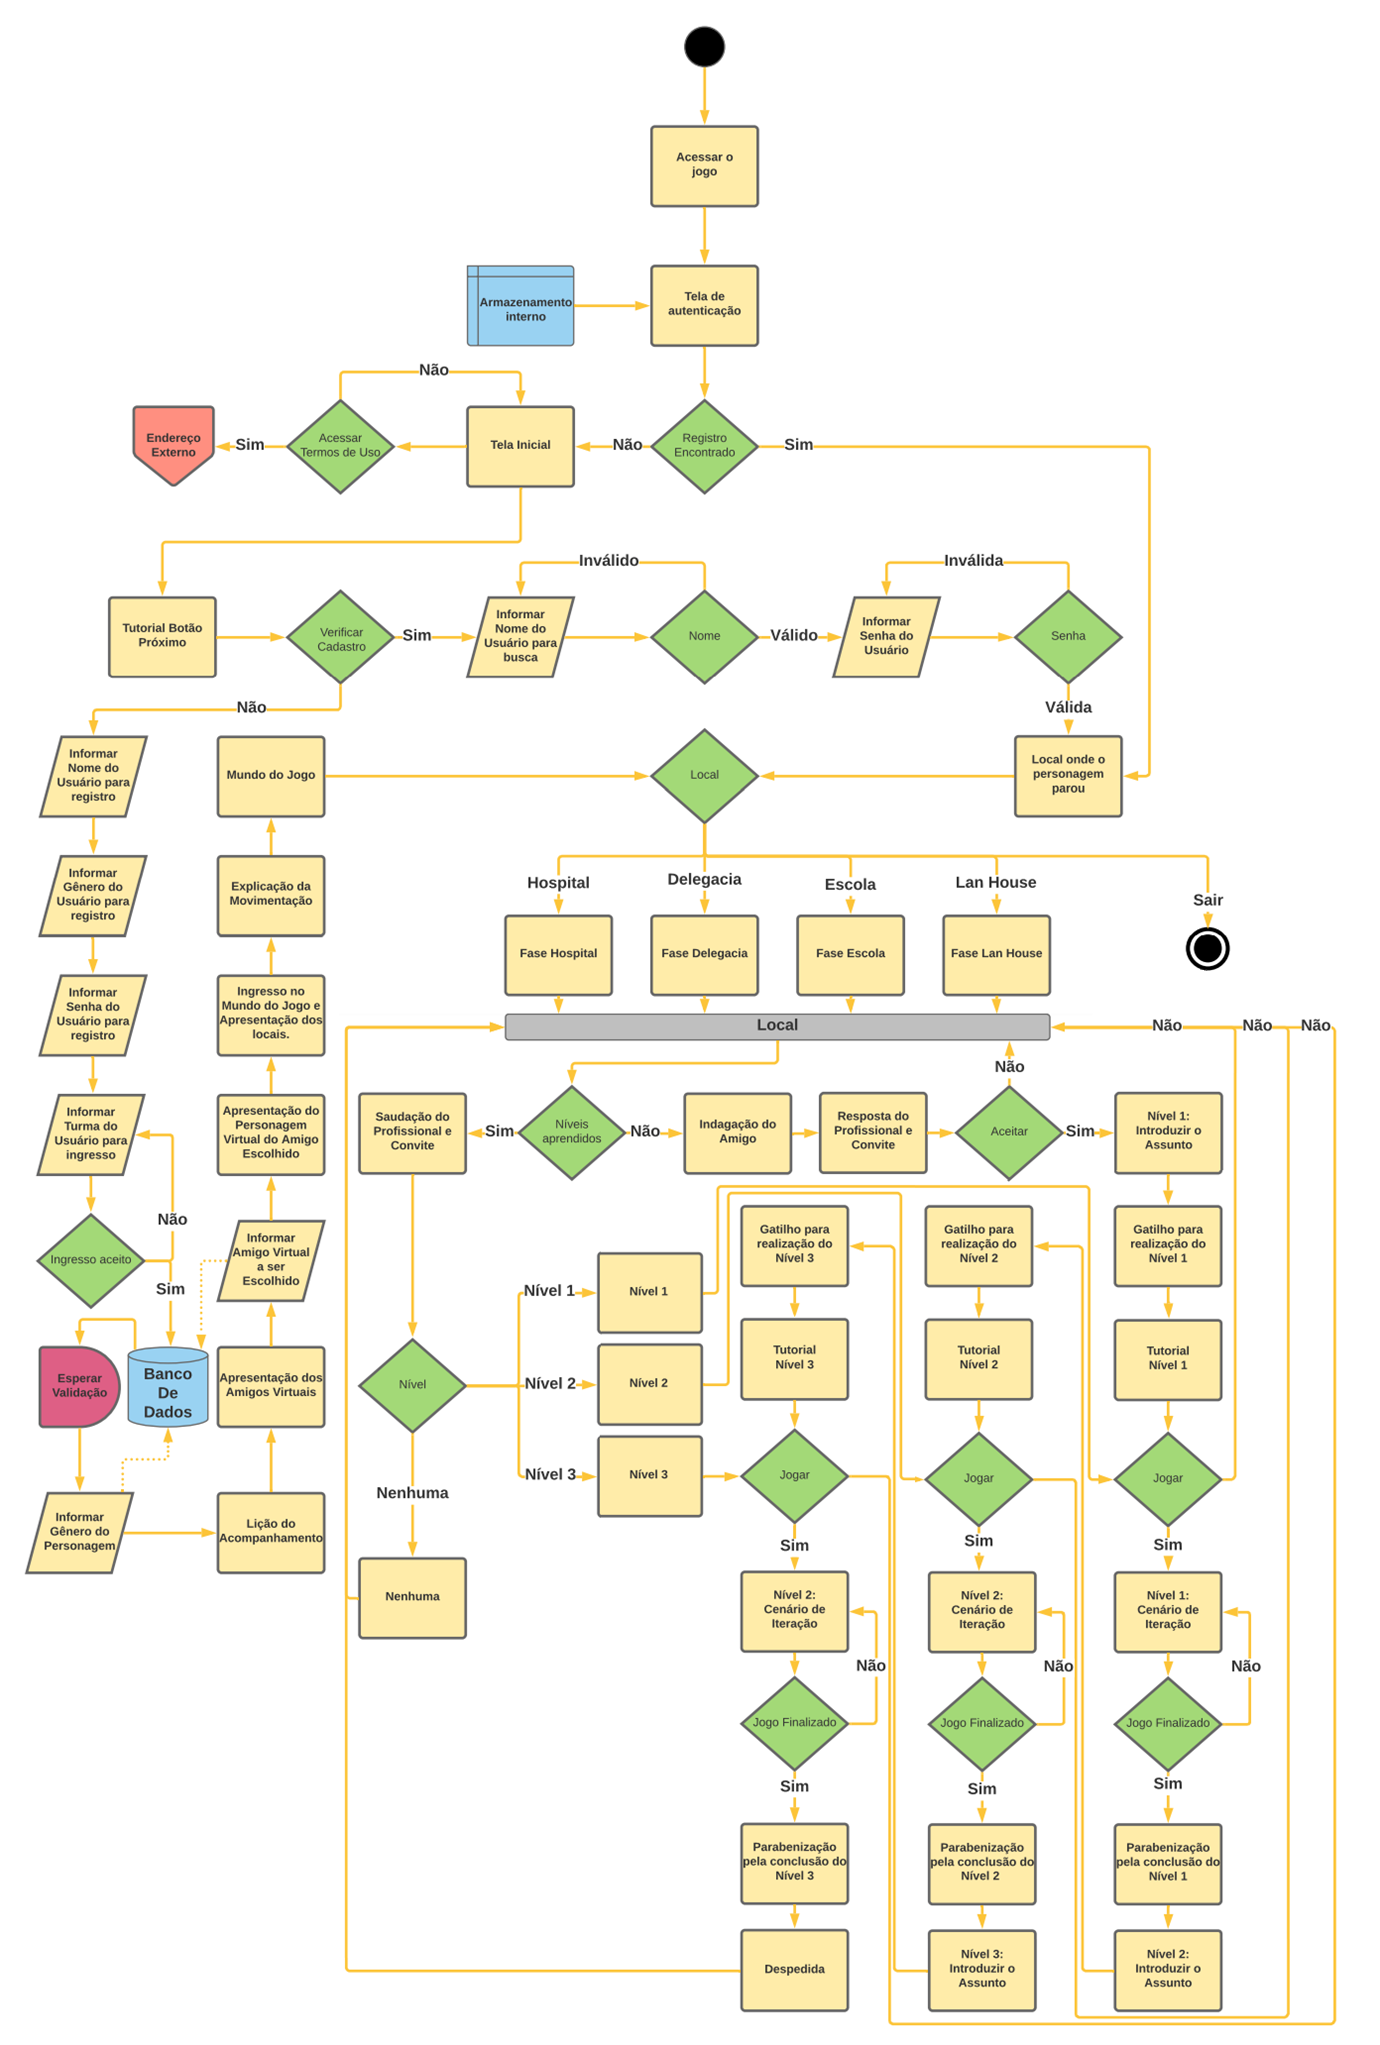
\includegraphics[width=0.95\linewidth]{./Figuras/DiagramaJoginho.png}
  \end{center}\vspace{-0.6cm}
\legend{Fonte: os autores}

\end{figure}


O diagrama de atividades da \autoref{fig:Diagrama}, representa de forma gráfica o fluxo de etapas necessárias para concluir cada atividade do jogo. A parte supeior corresponde as atividades relacionados ao acesso ao jogo. As atividades relacionadas ao cadastro no jogo é representados na parte esquerda do diagrama. Todas as demais atividades representadas no diagramas correspondem ao jogo em si. São quatro fases presentes no jogo: Fase do Hospital, Fase da Delegacia, Fase da Escola e Fase da Lan House. Cada fase possui três nível, em cada nível os jogadores aprendem conteúdos relacionados a prevenção da violência sexual infantil. 

\end{comment}

%O desconforto que imagens realistas poderiam causar no público e que fariam o jogo perder um pouco do caráter divertido. %https://www.sbgames.org/proceedings2020/ArtesDesignFull/209677.pdf (o fluxograma grama deles de ensinamentos é bem legal)

O jogo sério desta pesquisa visa ministrar assuntos sensíveis relacionados a sexualidade e a prevenção da violência sexual infantil. Por tal razão, todo o fundamental teórico do jogo advém de documentos devidamente revisados por especialistas na área de educação e sexualidade. Todo o conteúdo pedagógico do jogo é voltado para crianças de cinco até oito anos de idade. Os conteúdos selecionados para essa faixa etária seguem às orientações técnicas internacionais de educação em sexualidade \cite{women2018international}. Ainda no aspecto pedagógico, salienta-se que o jogo não se objetiva a utilizar figuras ou imagens realistas para apresentar um determinado conceito ou uma determinada situação. A literatura relata que a utilização de imagens reais de cunho sexual trazêm desconforto para alguns indivíduos, por tal razão toda a arte utilizada no jogo assume uma ilustração no estilo de um desenho infantil \cite{jogo2020Albert}.

%Jogos sérios devem balançear os aspectos didáticos e lúdicos do jogo. 

O jogo desenvolvido neste trabalho almeja a prevenção da violência sexual infantil. Embora a educação sexual seja o aspecto de maior presença no jogo, outras questões didático-pedagógicas ainda são levadas em consideração. Visando ajudar no letramento e na alfabetização das crianças, o jogo transcreve todos os diálogos na fonte \textit{Gill Sans}. A fonte \textit{Gill Sans} destaca-se com uma das melhores fontes para o desenvolvimento da leitura infantil \cite{lourencco2011tipografia}. 


%O jogo precisa agradar o público infantil com uma boa jogabilidade e bons desafios, na mesma medida que educa as crianças \cite{valenza2018guidelines}. Entre os aspectos que provocam engajamento do público infantil está a dublagem. No jogo desenvolvido, além da dublagem ser associada ao texto escrito existe a procupação com o letramento e alfabetização infantil. Por tal razão, os dialógos do jogo são escritos na fonte \textit{Gill Sans}.

O jogo sério desenvolvido possui uma estrutura metodológica de ensino baseada em quatro princípios a serem ministrados: Anatomia, Direitos, Denúncias e Ciberespaço. Cada um desses princípios se traduzem em uma fase no jogo, cada qual composta de três níveis. A \autoref{fig:conceitos} apresenta cada fase do jogo associada aos seus respectivos níveis.


\begin{figure}[hbt!]
  \caption{\label{fig:conceitos}Conceitos abordados}
  \begin{center}
    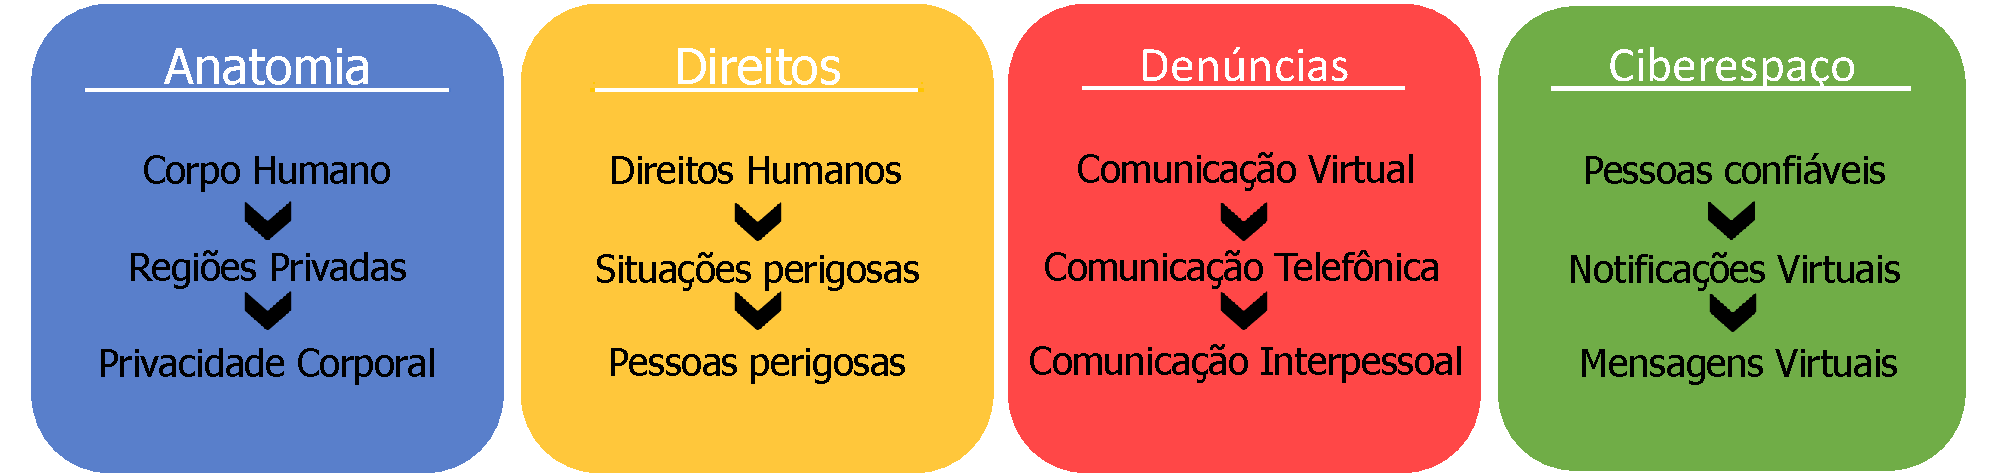
\includegraphics[width=\linewidth]{./Figuras/EsquemaFases.pdf}
    \end{center}
  \legend{Fonte: os autores}
  
\end{figure}

A \autoref{fig:conceitos} ilustra de maneira resumida cada um dos conteúdos a serem ministrados pelo jogo. Cada conteúdo é ministrado em um ambiente específico do jogo. Ou seja, o jogador possui liberdade de movimentação sobre o jogo, podendo alternar entre as fases da maneira que melhor lhe convir. Respectivamente, os conceitos sobre \textbf{Anatomia} são ministrados em um Hospital. Os direitos das crianças são ensinados em uma \textbf{Escola}. A realização de denúncias é um assunto ensinado em uma \textbf{Delegacia}. E a proteção no ambiente virtual das redes é ministrado em um \textbf{Cibercafé}.

A jogabilidade de jogo é flexível, permitindo ao jogador intercambiar entre as fases sem qualquer punição. Entretanto, os níveis das fases obedecem uma linearidade tanto de enredo, quando pedagógica (e.g. na fase da anatomia o jogador deve necessariamente aprender antes sobre os nomes das partes do corpo, para em seguida aprender quais são as partes íntimas do corpo, para por fim aprender os locais onde as pessoas podem tocar no corpo). O jogador tem liberdade para abandonar um nível sempre que desejar. Contudo, os últimos níveis são alcançáveis apenas após a conclusão dos anteriores. 

\newpage

O jogo apresenta aos jogadores conceitos sobre anatomia em um ambiente hospitalar. Três minijogos buscam ensinar aos jogadores questões sobre o Corpo Humano, Regiões Privadas e Privacidade Corporal. A \autoref{fig:Hospitalzinho} ilustra as dinâmicas utilizadas em cada um dos minijogos. Todos os conceitos desse ambiente são ministrados pelo personagem de um médico. 


\begin{wrapfigure}[29]{r}{7.0cm}%pulando 29 linhas
  \vspace{-20pt}
  \caption{\label{fig:Hospitalzinho}Hospital}
  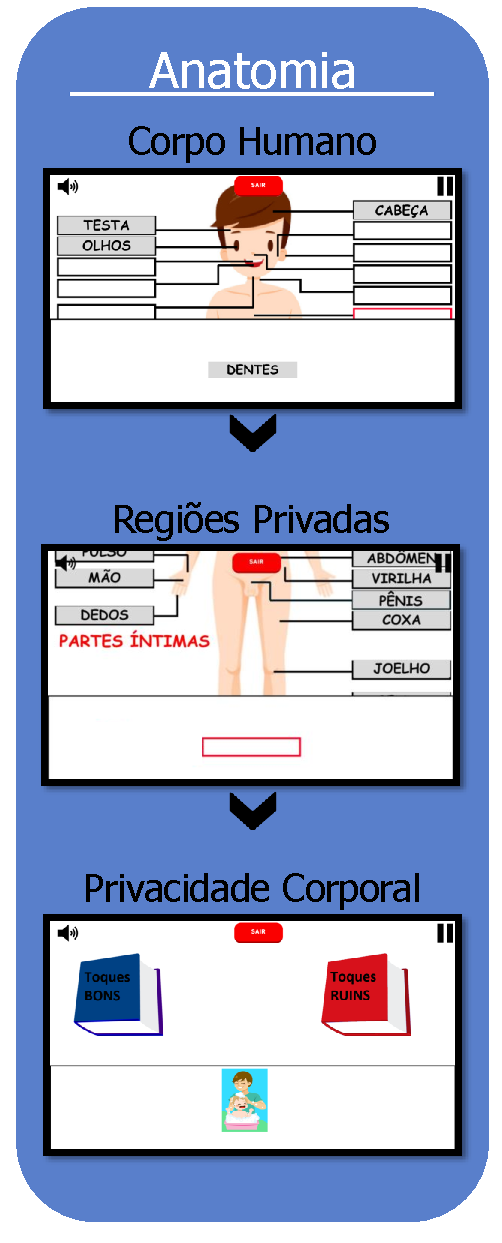
\includegraphics[width=\linewidth]{./Figuras/Hospital.pdf}
  \vspace{-1.0cm}
  \legend{Fonte: os autores}
\end{wrapfigure}

O primeiro nível (Corpo Humano) busca ensinar ao jogador o nome correto das partes do corpo humano. O médico apresenta as partes do corpo em um mural do corpo humano masculino e feminino. Após o jogador ser ensinado sobre as partes do corpo, algumas peças do mural caem. O jogador deve então nessa etapa, demonstrar seus conhecimentos sobre o corpo humano, inserindo as peças em suas respectivas posições. As peças vão aparecendo uma a uma no centro da caixa de diálogo, sendo que o jogador deve arrastá-las e movê-las para suas posições. %originais. 


O segundo nível (Regiões Privadas) busca ensinar ao jogador as partes íntimas do corpo humano. O médico educa o jogador sobre as zonas privadas e não privadas do corpo no mesmo mural do primeiro nível. As regiões privadas são representadas por peças com contorno vermelho no mural. Após o jogador ter adquirido esse conhecimento, os contornos vão ao chão. Neste momento o jogador deve levar os contornos vermelhos para as peças que representam as partes íntimas.

O terceiro nível (Privacidade Corporal) busca ensinar ao jogador sobre os toques bons e os toques ruins. O médico apresenta para isso dois livros, um apenas com imagens de toques bons e outro apenas com imagens de toque ruins. Ao fechar o livro as páginas se desprendem e as imagens se misturam. O jogador deve então demonstrar seus conhecimentos classificando devidamente as imagens. As imagens vão aparecendo uma por uma na caixa de diálogo, com o jogador tendo que movê-las para seus respectivos livros. 

O jogo desenvolvido neste trabalho apresenta aos jogadores seus direitos e deveres. Três minijogos buscam ensinar aos jogadores questões sobre Direitos Humanos, Situações Perigosas e Pessoas Perigosas. A \autoref{fig:Escola} ilustra as dinâmicas utilizadas em cada um dos minijogos. Todos os conceitos desse ambiente são ministrados pelo personagem de uma professora. 

\begin{wrapfigure}[29]{r}{7.0cm}%pulando 29 linhas
  \vspace{-20pt}
  \caption{\label{fig:Escola}Escola}
  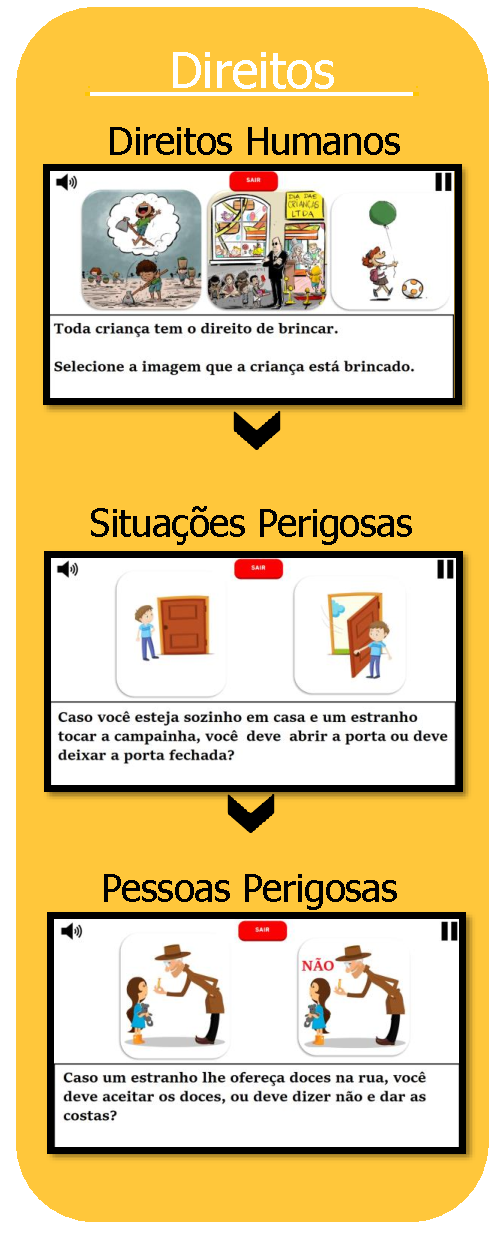
\includegraphics[width=\linewidth]{./Figuras/Escola.pdf}
  \vspace{-1.0cm}
  \legend{Fonte: os autores}
\end{wrapfigure}

O primeiro nível (Direitos Humanos) busca ensinar ao jogador sobre os direitos da criança no Brasil e no mundo. A professora discorre sobre os direitos e deveres das crianças pedindo para o jogador selecionar a imagem que mais representa um determinado conceito. O jogador então além de ser ensinado verbalmente e textualmente sobre seus dinheiros, demonstra seus conhecimentos em uma representação visual. Tal método de ensino, demonstra a capacidade de abstração da criança ao criar uma imagem mental dos conceitos aprendidos e associar essa imagem mental a uma figura no jogo. 

O segundo nível (Situações Perigosas) visa educar o jogador sobre sua segurança. O jogador é ensinado que as crianças não estão totalmente protegidas de seus direitos e por isso é importante tomar cuidado com determinadas situações que podem colocar as crianças em risco, na qual os direitos das crianças seriam desrespeitados. Um conjunto de situações é apresentado ao jogador onde o jogador deve optar em escolher duas situações. Nesse jogo de perguntas e respostas o jogador deve então demonstrar que sabe evitar situações potencialmente perigosas.

O terceiro nível (Pessoas Perigosas) busca ensinar ao jogador sobre pessoas que podem desrespeitar os direitos das crianças. A professora realiza um jogo de perguntas e respostas similar ao jogo do segundo nível, porém ao invés de apresentar situações, pessoas são apresentadas. Nesse jogo, o jogador deve então demonstrar que sabe evitar pessoas que apresentem atitudes potencialmente perigosas.


O jogo sério deste trabalho apresenta aos jogadores formas nas quais são possíveis formalizar uma denúncia. Três minijogos buscam ensinar aos jogadores questões relacionadas a Comunicação Virtual, Comunicação Telefônica e Comunicação Interpessoal. A \autoref{fig:DelegaciaDP} ilustra as dinâmicas utilizadas em cada um dos minijogos. Todos os conceitos desse ambiente são passados pelo personagem de um delegado. 

\begin{wrapfigure}[29]{r}{7.0cm}%pulando 29 linhas
  \vspace{-20pt}
  \caption{\label{fig:DelegaciaDP}Delegacia}
  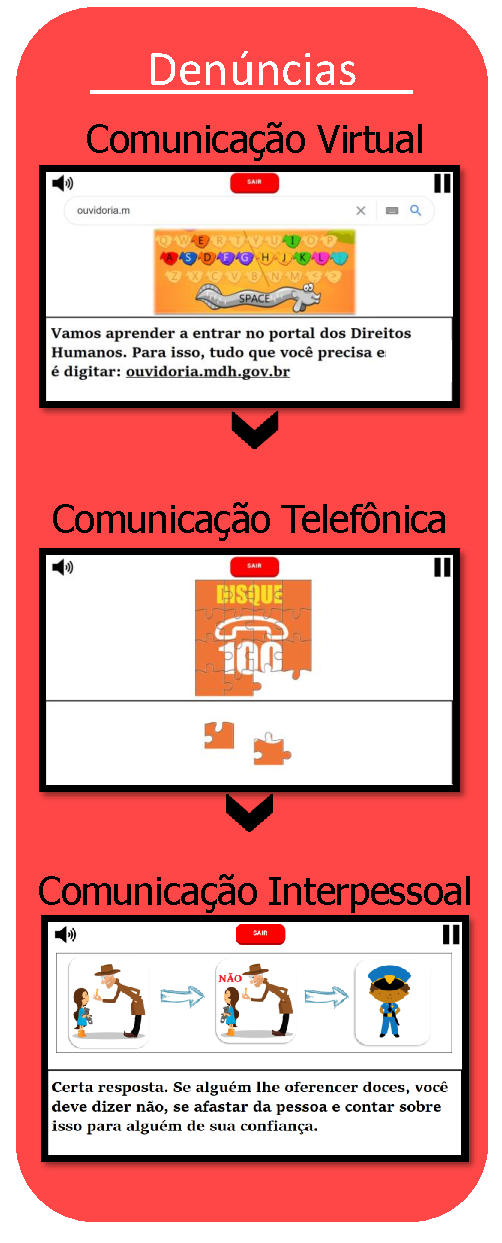
\includegraphics[width=\linewidth]{./Figuras/Delegacia.pdf}
  \vspace{-1.0cm}
  \legend{Fonte: os autores}
\end{wrapfigure}

O primeiro nível (Comunicação Virtual) busca ensinar ao jogador formas nas quais o jogador pode realizar uma denúncia pela \textit{Internet}. O delegado apresenta então um computador onde um jogo de datilografia se inicia. Nesse jogo, o jogador é instruído a pesquisar e digitar corretamente os canais de denúncia nacional. O jogo é pensado de forma a ser acessível para as crianças que não encontram-se totalmente alfabetizadas. 

O segundo nível (Comunicação Telefônica) ensina ao jogador sobre as linhas telefônicas para a denúncia de crimes contra a criança. O delegado apresenta no interior da delegacia um mural com um número telefônico. Após o jogador visualizar o mural, os elementos do mural vão ao chão. Em um jogo de quebra-cabeça o jogador deve então montar novamente o mural. A dinâmica lúdica utilizada neste jogo, prolonga o contato do jogador com o canal de denúncia do Disque 100, ampliando assim a retenção da informação. 

O terceiro nível (Comunicação Interpessoal) busca ensinar ao jogador como realizar denúncias pessoalmente. O delegado apresenta para isso um livro ilustrando algumas situações. As situações ilustradas representam eventos e a passagem entre os eventos (tempo) é representada por setas. Ao fechar o livro as ilustrações se desprendem e vão ao chão. Neste momento o jogador é confrontado a montar novamente a ordem dos acontecimentos (eventos) ilustrada no livro. O jogador então demonstra como se comportar em um conjunto de situações e como relatar a ordem dos acontecimentos para uma pessoa confiável. 

O jogo apresenta as maneiras como se proteger nas redes. Três minijogos buscam ensinar aos jogadores questões sobre Pessoas Confiáveis, Notificações Virtuais e Mensagem Virtuais. A \autoref{fig:Cibercafe} ilustra as dinâmicas utilizadas em cada um dos minijogos. Todos os conceitos desse ambiente são ministrados pelo personagem de um robô. 


\begin{wrapfigure}[29]{r}{7.0cm}%pulando 29 linhas
  \vspace{-20pt}
  \caption{\label{fig:Cibercafe}Cibercafé}
  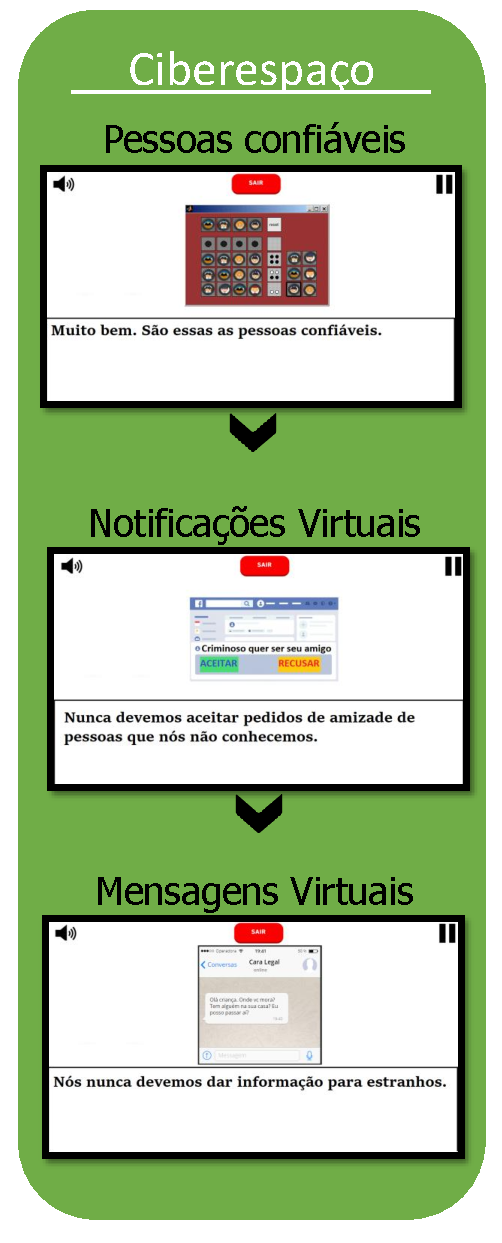
\includegraphics[width=\linewidth]{./Figuras/Cibercafe.pdf}
  \vspace{-1.0cm}
  \legend{Fonte: os autores}
\end{wrapfigure}

O primeiro nível (Pessoas Confiáveis) busca ajudar o jogador a identificar pessoas de confiança. O robô do cibercafé conta que perdeu a senha do computador, mas sabe que a senha é um conjunto de fotos das pessoas que ele confia. A dinâmica de jogo consiste na tentativa e erro do jogador em montar um conjunto de pessoas de confiança até atingir a combinação correta. Durante esse nível as escolhas certa e erradas são justificadas ao jogador, ajudando a compreender o que define uma pessoa de confiança ou não. 

O segundo nível (Notificações Virtuais) busca ensinar ao jogador como se comportar nas redes sociais. O robô enfatiza da importância das redes sociais e salienta que crianças menores de 13 anos não deveriam usar redes como o \textit{Facebook}. Contudo, caso usem o robô explica do cuidado em adicionar apenas pessoas conhecidas e também avisa sobre a existência de perfis falsos se passando por pessoas conhecidas. A dinâmica do jogo deste nível consiste no jogador aceitar e recursar devidamente pedidos de amizade, além de aprender a desfazer amizades. %(caso um erro seja cometido). 

O terceiro nível (Mensagens Virtuais) busca ensinar ao jogador como se comunicar na \textit{Internet}. O robô explica que alguns serviços de mensagem instantânea como o \textit{Whatsapp} também possuem uma idade mínima para uso de 13 anos de idade, porém diferente do \textit{Facebook} qualquer pessoa pode lhe enviar uma mensagem sem sua prévia autorização. A dinâmica do jogo consiste em ensinar o jogador a não compartilhar informações com estranhos, além de bloqueá-los e relatar os acontecimentos para um adulto. %de confiança. 


\begin{comment}
propósito

Orientações em Sexualidade

Plataforma

Publico Alvo

Estilo

Estética

Arte

Fonte

Escalabilidade/Flexibilidade

Audio

Musica

Leiaute de Níveis

UX

Gamificação

Ergonomia de Botões

Artefato

Licença

Termos de Serviço

Política de Privacidade

Criptografia

Banco de Dados
\end{comment}

O jogo sério desenvolvido por este trabalho é constituído por doze minijogos voltados a educar os jogadores sobre questões relacionadas a temática da violência sexual infantil. Todos os minijogos, independentemente de sua fase, apresentam a mesma Barra de Estado, como pode ser observado nas telas do jogo das Figuras \ref{fig:Hospitalzinho}, \ref{fig:Escola}, \ref{fig:DelegaciaDP} e \ref{fig:Cibercafe}. A Barra de Estado (HUD - Head-Up Display), é uma região da tela do jogador na qual informações ou elementos são dispostos de modo a não atrapalhar a visão do jogador, sendo anexados normalmente nas extremidades da tela. Os elementos da Barra de Estado do jogo são um botão para silenciar/desilenciar o jogo (canto superior direito), um botão para parar/desparar o jogo e um botão vermelho para sair dos minijogos (centro superior). O botão vermelho situado na região superior de todos os doze minijogos é um botão presente apenas nestes momentos. Quando o jogador está transitando entre os ambientes do jogo, o botão não é apresentado. 

%pois para sair do jogo como um todo, o jogador precisa apenas encerra a aplicação. No entanto, para sair dos minijogos, basta apenas clicar no botão vermelho.

Todas as ações realizadas pelos jogadores durante as dinâmicas ministradas no jogo são enviadas para um banco de dados relacional. Dados sobre a quantidade de acertos e erros preenchem os campos no banco de cada um dos jogadores. Os dados gerados pelo sistema não são apresentados ao jogador em nenhum momento. As informações coletadas servem para compreender melhor o desempenho dos jogadores e suas preferências. O jogo opera unicamente em navegadores, necessitando de uma conexão com a \textit{Internet} para ser carregado no navegador. A conexão com a \textit{Internet} ainda se faz necessária durante os minijogos, pois são durante estes momentos que o jogo realiza requisições ao banco de dados. 

%O jogo desenvolvido encontra-se hospedado publicamente. Salienta-se nesse sentido que até a data de publicação deste trabalho a corrente versão do jogo encontra-se inacabada. Desta forma, não se recomenda que o jogo seja ministrado para crianças até a formulação de uma versão mais robusta e acabada do jogo. Sua disponibilização ao público objetiva-se apenas em uma publicação mais detalhada dos frutos da presente pesquisa. Dito isso, o jogo em questão encontra-se hospedado na plataforma de desenvolvimento de aplicativos para dispositivos móveis \textit{Firebase} da empresa multinacional de serviços \textit{Google}, sendo acessível pelo seguinte endereço da \textit{internet}: \url{https://infancia.firebaseapp.com/}




%%%%%%%%%%O enredo é tão importante para jogos sérios como não-sérios, pois permite que o jogador se projete na personagem do jogo (McDaniel et al., 2010). [tese Adilson] = Falar da dinâmica do herói mudo.


%Digital Natives. Our students today are all “native speakers” of the digital language of computers, video games and the Internet. %https://www.marcprensky.com/writing/Prensky%20-%20Digital%20Natives,%20Digital%20Immigrants%20-%20Part1.pdf %https://colegiongeracao.com.br/novageracao/2_intencoes/nativos.pdf


%Para que um game seja completo, e atenda a critérios de usabilidade, é essencial promover algum mecanismo que facilite o aprendizado do funcionamento do jogo. De acordo com Squire et al. (2005, p.41), mediadores são fundamentais nos primeiros dias%https://www.udesc.br/arquivos/cct/id_cpmenu/1024/diego_buchinger__1__15167055468902_1024.pdf


%A Metodologia Institucional “Aprender na Prática”, que prevê “a ação educativa na participação ativa e crítica do aluno em sua aquisição de conhecimentos práticos e teóricos” [UNICSUL, 2004] 


%desenvolvimento solitário baseado em ambiarra (DSBA)